\chapter{Resultat}

\section{Installation av systemet}
Ett av kraven från kunden var att kunna installera systemet på sin egna server
och låta det köra därifrån. För att underlätta för kunden vid installationen
skapades en installationsfil som laddar ner systemets filer, fixar inställningar
för databasen och även ställer frågor om vilka tredjepartstjänster som ska
användas. Installationsfilen anpassar sedan systemet utefter de svar som fås av
användaren vid installation. Stegen demonstreras i bild \ref{fig:installation}.

\begin{figure}[!h]
\centering
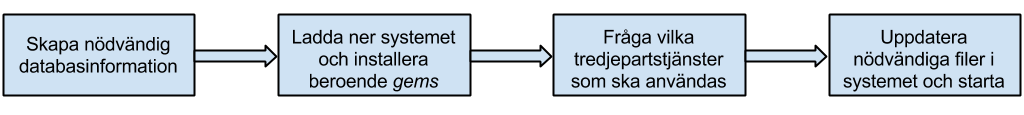
\includegraphics[width=0.8\textwidth]{figures/installation.png}
\caption{De steg som installationsfilen tar för att installera systemet.}
\label{fig:installation}
\end{figure}

\section{Systemarkitektur}

\subsection{Ruby on rails}
Följande modeller valdes att användas för systemet. Relationerna mellan de är
specificerade i bild \ref{fig:models}. Modellen \emph{BruseFile} fick det namnet
eftersom \emph{File} är ett reserverat ord i Ruby och lösningen blev då att
lägga till \emph{bruse}.

\begin{figure}[!h]
\centering
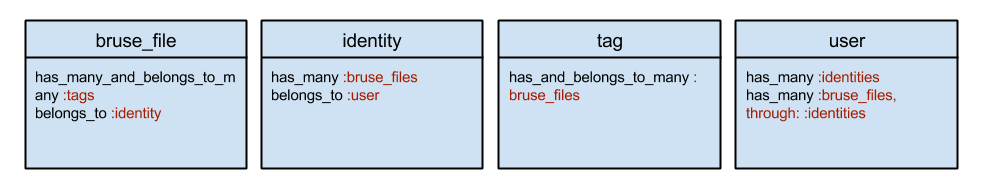
\includegraphics[width=0.8\textwidth]{figures/models.png}
\caption{De \emph{models} som finns i systemet.}
\label{fig:models}
\end{figure}

\emph{Identity} är en av  systemets viktigaste models. En \emph{Identity} är
antingen en av tredjepartstjänsterna Google Drive eller Dropbox. Men även den
egna filhantering hanteras som en \emph{Identity} för att hålla det konsekvent
och modulärt.

För att kunna presentera en fil och dess taggar äger \emph{BruseFile} flera
taggar, men för att även kunna lista filer beroende på en tagg äger varje tagg
flera \emph{BruseFiles}. Rails löser relationen mellan dessa två genom att skapa
en tabell som heter \emph{bruse\_files\_tags} enligt bild
\ref{fig:bruse_files_tags}.

\begin{figure}[!h]
\centering
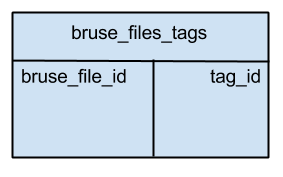
\includegraphics[width=0.2\textwidth]{figures/bruse_files_tags.png}
\caption{Relationen mellan \emph{BruseFiles} och \emph{tags} i databasen.}
\label{fig:bruse_files_tags}
\end{figure}

I systemet finns det flera \emph{controllers} för att hantera logiken. Varje
\emph{model} har en \emph{controller}, men \emph{bruse\_file} delades upp i tre
då den innehåller all logik kring uppladdning, nerladdning, visa filer, lista
med mera.

\subsection{Angularjs}
De områden som styrs utav Angularjs är:
\begin{itemize}
  \item Lägga till filer
  \item Lägga till taggar till nyligen tillagda filer
  \item Söka efter filer
  \item Skapa filer från text
  \item Dra och släppa-uppladdning
  \item Lista filer
\end{itemize}

För att inte behöva upprepa kod, för till exempel hämta information kring filer,
skapades factories för att kunna delas utav flera \emph{controllers}, där finns
logik och rätt parametrar för att kunna skicka en \emph{AJAX}-förfrågan till
servern.

\section{Tredjepartsmjukvara}

Devise är ett tillägg till Ruby on rails som ger ett paket för
användarhantering, färdigt att användas. Då beslutet om att användare även
skulle kunna logga in med e-postadress och lösenord insågs det samtidigt att en
tredjeparts-tjänst skulle vara nödvändigt för att hålla tidsramen. Devise valdes
för att det gav den mest kompletta lösningen med färdiga vyer, modifierbara
\emph{controllers} och enkel \emph{model}-påbyggnad.

Carrierwave ger utvecklarna verktyg för att hantera uppladdningen av filer.
Genom att endast specificera inställningar för var filen ska sparas och så
vidare fås en modul som kan användas i de \emph{controller}-metoder som behövs.

Fuzzily skapar för varje ny instans av specificerade \emph{models}
\emph{trigrams} över valda kolumner. \emph{Trigrams} delar upp en instans och
grupperar dem tre i taget. För varje ny gruppering förflyttas den ett steg
vilket gör att det skapas flera olika kombinationer. För ett ord skulle det
resultera i flera olika bokstavskombinationer av grundordet. Exempelvis skulle
ordet “bruse” med hjälp av \emph{trigrams} bli [b, br, bru, rus, use, se, e].
Under implementationen av Fuzzily märktes att numeriska eller nordiska tecken
inte blev till \emph{trigrams}. Men då Fuzzily är open source kunde problemet
åtgärdas genom att ändra källkoden.

Jstag är ett tillägg till Angularjs som konverterar användarens inskrivning utav
taggar till visuella objekt för att tydliggöra för användaren hur dess
inskrivning tolkas utav systemet. Även detta tillägg hade brister i koden som
kunde åtgärdas tack vare att det var skrivet med öppen källkod.

\section{Hantering och strukturering av databaser}

Den första versionen av databasen hade följande struktur:
\begin{itemize}
\item User
  \begin{itemize}
    \item id (heltal, unik nyckel)
    \item name (sträng, användarens namn)
  \end{itemize}
\item Identity
  \begin{itemize}
    \item id (heltal, unik nyckel)
    \item user\_id (heltal, referens till användare)
    \item service (sträng, till exempel “Dropbox”)
    \item token (sträng, nyckel som används för kontakt med extern API)
  \end{itemize}
\item File
  \begin{itemize}
    \item id (heltal, unik nyckel)
    \item identity\_id (heltal, referens till identity)
    \item name (sträng, filens namn)
    \item foreign\_ref (sträng, hur den externa tjänsten har koll på filerna)
    \item filetype (sträng, filens typ)
    \item meta (sträng, extra information om filen)
  \end{itemize}
\item Tag
  \begin{itemize}
    \item id (heltal, unik nyckel)
    \item name (sträng, nyckelordet)
  \end{itemize}
\item FileTag
  \begin{itemize}
    \item file\_id (heltal, referens till fil)
    \item tag\_id (heltal, referens till nyckelord)
  \end{itemize}
\end{itemize}

\section{Filhantering}

Då en fil lagrades i systemet är det två attribut som var centrala. Dels
varifrån filen sparats – om den importerades från en extern tjänst som Google
Drive eller Dropbox, eller om den lagrades i systemets lokala fillagring. Vidare
sparas också en textsträng som motsvarar hur den aktuella tjänsten som filen
tillhör håller koll på filen. Denna textsträng kallas i systemet för
\emph{foreign\_ref}. För Google Drive är detta en slumpmässig bokstavs- och
sifferkombination, för Dropbox är detta sökvägen till filen. För den lokala
filhanteringen är detta namnet på filen efter att den sparats på servern, också
detta en slumpad bokstavs- och sifferkombination.

\section{Gränssnitt}

\section{Testning}

De tester som utvecklarna lade mest tid på att implementera var tester för
\emph{models}, \emph{controllers} men även integrationstester.
Integrationstester är tester som testar ett användarbeteende och har väldigt
enkla instruktioner, till exempel gå till startsidan och fyll
inloggningsformuläret med dessa uppgifter och tryck sedan på logga in. Med dessa
tester fås en helhetsblick och väldigt stor del av systemet testas i ett och
samma test.

För kunna testa viss funktionalitet krävs data i databasen, för detta har
Minitest något som heter Fixtures. Det är data som man kan fejka och Minitest
hanterar sedan dessa som databasinlägg.

\section{Utvecklingsmetodik}

Arbetet följde Scrum som utvecklingsmetodik vilket har resulterat i en tydlig
och strukturerad arbetsgång. Korta Scrummöten i början av varje arbetsdag har
förhindrat onödigt arbete samt att alla utvecklare är insatta i arbetet. Varje
sprints sprintgranskning och sprintåterblick har givit en tydlig bild om vad som
gjorts och behöver göras för att nå nästa förbättring av produkten.

\section{Versionshantering och kodgranskning}
